\section{Problem 2}

\subsection{Question}
\vspace*{10pt}
Determine if the friendship paradox holds for your Twitter account.
Since Twitter is a directed graph, use \enquote{followers} as value you measure 
$($i.e., \enquote{do your followers have more followers than you?}$)$.\\
\\
Generate the same graph as in question \#1, and calcuate the same 
mean, standard deviation, and median values.\\
\\
For the Twitter 1.1 API to help gather this data, see:
\\
\url{https://dev.twitter.com/docs/api/1.1/get/followers/list}
\\
If you do not have followers on Twitter (or don't have more than 50),
then use my twitter account \enquote{phonedude\_mln}.

\subsection{Answer}
Using Dr. Michael Nelson's Twitter account and the Twitter API \cite{api:twitter}, specifically the GET friends/list \cite{api:twitter_followerslist} request, all of Dr. Nelson's Twitter friends were obtained and saved to the file called {\tt followers}. This method also uses the API's paginating scheme: when there are a large number of results for a query, the API will send a cursor index to show that there are more results to process and that more requests are needed. The code to do this is in Listing \ref{listing:get_followers}. 

\lstinputlisting[language=Python, caption={get\_followers.py}, label=listing:get_followers]{q2/get_followers.py}

\clearpage
To reduce the impact of high HTTP traffic, the Twitter API rate-limits most requests -- the one needed to obtain a user's friends list has a limit of fifteen message per fifteen minutes. Any requests received from a user or service that has reached the limit will be denied.
\\
The friends of Dr. Nelson's friends were then obtained with the same {\tt get\_followers} method from Listing \ref{listing:get_followers} and stored in a file called {\tt followers\_counts}, each on a single line preceded by their friend count. All of these operations were controlled by a main method, which is shown in Listing \ref{listing:get_followers}.
\\
The {\tt followers\_counts} file was ordered in place with the Unix command in Listing \ref{listing:sort1}. 
\vspace{2mm}
\begin{lstlisting}[language=Bash,caption={Sort command},label=listing:sort1]
Naina Sai Tipparti@DESKTOP-2FU7AJC ~/a4/q3 cat followers_counts | sort -g -o followers_counts
\end{lstlisting}
\vspace{2mm}
This file was then processed by the R script shown in Listing \ref{listing:followers_graphr} to produce the graph in Figure \ref{fig:followers_graph}

\lstinputlisting[language=R, caption={Graph Creation Script for Twitter}, label=listing:followers_graphr]{q2/plot_followers.R}

\clearpage
The median, mean and standard deviation were all calculated, with the median, mean and median plus one standard deviation.
\vspace*{2mm}
\begin{table}
\centering
\begin{tabular}{ l l }
\hline
\textbf{Mean} & 1024.7424 \\
\textbf{Median} & 258 \\
\textbf{Std Dev} & 4135.7974\\
\hline
\end{tabular}
\caption{Statistics on the count of Dr.Nelson Followers, values straight from R}
\label{tab:q1stats}
\end{table}
\begin{figure}[h!]
\centering
\fbox{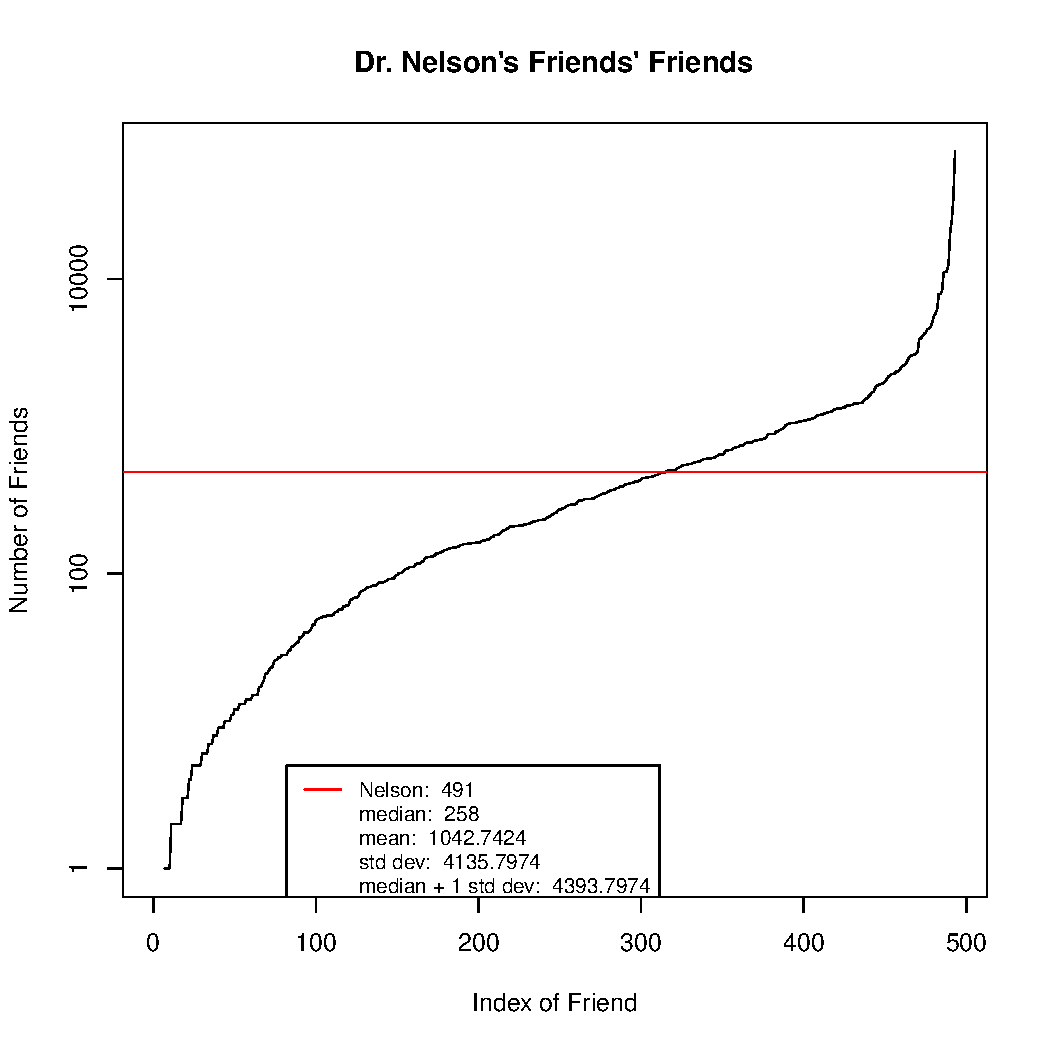
\includegraphics[scale=0.75]{q2/followers_plot.pdf}}
\caption{The Friendship Graph for Twitter Followers}
\label{fig:followers_graph}
\end{figure}


